\chapter{Realisierung}

Im folgenden Abschnitt soll auf die Implementierung des \textit{Smart Warehouse} Szenarios eingegangen werden. Insbesondere werden Probleme während der Umsetzung der beiden Objektdetektoren \textit{SSD} und \textit{YOLO} betrachtet, Herausforderungen im Rahmen der Drohnen Anbindung besprochen und letztendlich die Realisierung der Dashboard-Webapplikation zur Durchführung der Inventur aufgezeigt. 

\section{Umsetzung der Objektdetektoren}

\subsection*{SSD}

Für den \textit{SSD} wurde wie bereits erläutert nicht die ursprüngliche Referenzimplementierung im \textit{Caffe} Framework verwendet, sondern eine Custom-Implementierung in \textit{PyTorch}. Da der erstellte Datenbestand nur 1078 gelabelte Daten enthält, wurde zusätzlich zur Custom-Implementierung ein fünffaches Kreuzvalidierungsverfahren realisiert. Es dient dazu ein höheres Abstraktionsvermögen des Modells auf dem geringen Datenbestand zu erreichen. Auch unterstützte die Referenzimplementierung keine Validierung durch zuvor ungesehene Daten. Die Modellklassen zur Abstraktion des Datenbestandes wurden dahingehend angepasst.

Um ein lokales Training auf der \textit{NVIDIA GTX 1080} GPU zu ermöglichen, wurde zudem \textit{CUDA} Version 10.1 verwendet. Trainiert wurde mit folgenden Hyperparametern:
\begin{itemize}
	\item Batch Größe: 16
	\item Lernrate: $1.0\cdot e^{-3}$
	\item Momentum: 0.9
	\item Epochen: 500
	\item Gradientenverfahren: Stochastic Gradient Descent
	\item Kostenfunktion: Smooth L1
\end{itemize}

Das Basisnetzwerk des \textit{SSDs} besteht aus einem auf \textit{ImageNet} vortrainierten \textit{VGG16}. Die restlichen \textit{Convolutional Layer} sind \textit{Xavier} initialisiert. 

Die Hyperparameter sind nahezu gleich zu denen in der ursprünglichen wissenschaftlichen Veröffentlichung. Wesentlich die Batch Größe wurde für größere Stabilität von 32 auf 16 heruntergesetzt. Auch in der Evaluierung wurde die Batch Größe von 64 auf 48 herunter gesetzt, da die Eingangsdaten eine weitaus höhere Auflösung als die ursprünglich im \textit{PascalVOC} verwendeten Daten haben. Andernfalls wird Gefahr gelaufen einen Speicherüberlauf zu erzielen. 

Ursprünglich wurden 500 Epochen für das Training vorgesehen für jeden der Kreuzvalidierungsschritte. Da allerdings beim Training schon nach knapp über hundert Epochen sich der Gradient der Kostenfunktion nur träge veränderte, wurde im Sinne des \textit{Early Stoppings} nach 108 Epochen das Training vorzeitig beendet, um \textit{Overfitting} zu vermeiden. Das niedrigste Ergebnis der Kostenfunktion betrug 1.726. Es ergab eine \textit{mAP} von 78.2\%, leicht über den Referenzergebnissen von \textit{PascalVOC}. 

Wird nun das trainierte Modell auf echte Daten angewendet, so fällt auf, dass manche Objekte doppelt detektiert werden. Um dieses Problem zu lösen, gibt es zwei Möglichkeiten. 

Als erstes kann bei der Detektion der minimale \textit{confidence score} angegeben werden, ab wann eine Detektion offiziell als solche wahrgenommen wird. Hier liegt die Herausforderung darin, einen optimalen Wert zu finden, sodass verdeckte Objekte noch als solche erkannt werden, aber doppelt erkannte Objekte nicht mehr auftreten. Der \textit{confidence score} wurde nach mehrmaligem Iterieren auf 0.75 festgelegt.

Die zweite Möglichkeit besteht darin, die maximale Überlappung zweier Bounding Boxen festzulegen. Somit werden doppelte Bounding Boxen, die sich flächenmäßig über einem gewissen Grenzwert überlappen, auf eine Bounding Box reduziert. Er stellte ich sich Parameter von 0.5 als geeignet heraus.

Außerdem wurden Inkonsistenzen im Detektionsverhalten festgestellt:

\begin{figure}[htbp]
	\begin{minipage}[t]{8cm}
		\vspace{0pt}
		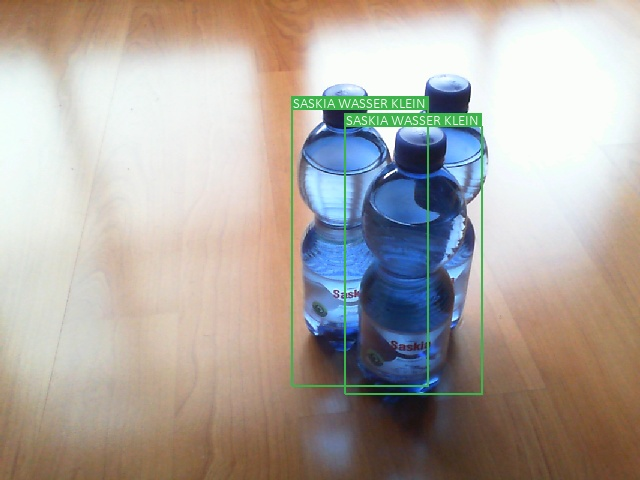
\includegraphics[width=7cm]{Bilder/double.jpeg}
		\caption[Detektion mehrerer Wasserflaschen]{Detektion mehrerer Wasserflaschen}
		\label{double}
	\end{minipage}
	\hfill
	\begin{minipage}[t]{8cm}
		\vspace{0pt}
		\begin{onehalfspace}
			So ist es schwierig, teilweise verdeckte Objekte zu detektieren (siehe Abbildung \ref{double}). Dies mag aber auch daran liegen, dass im Trainingsdatensatz nicht genügend Daten vorhanden waren, die solche Fälle abdecken. Auch die Detektion von entfernteren Objekten gestaltete sich gegenüber näheren Objekten schwieriger (siehe Abbildung \ref{near} und \ref{far})
		\end{onehalfspace}
	\end{minipage}
\end{figure}

\begin{figure}
	\begin{minipage}[b]{.45\linewidth} % [b] => Ausrichtung an \caption
		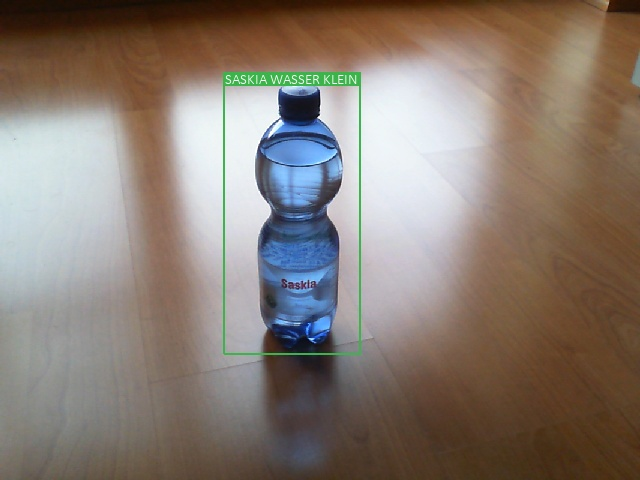
\includegraphics[width=\linewidth]{Bilder/near.jpeg}
		\caption[Detektion einer nahen Wasserflasche]{Detektion einer nahen Wasserflasche}
		\label{near}
	\end{minipage}
	\hspace{.1\linewidth}% Abstand zwischen Bilder
	\begin{minipage}[b]{.45\linewidth} % [b] => Ausrichtung an \caption
		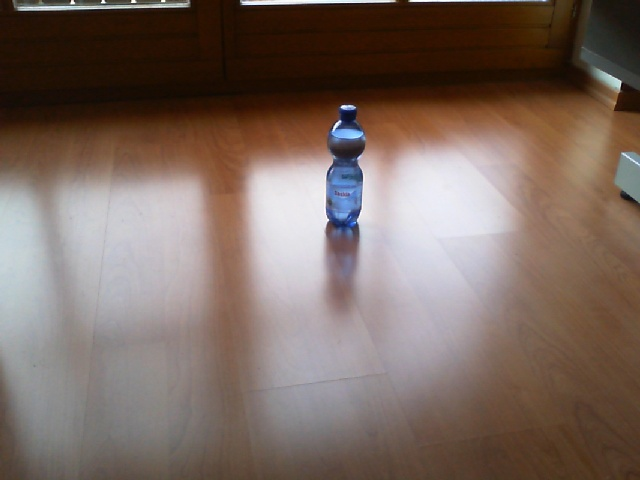
\includegraphics[width=\linewidth]{Bilder/far.jpeg}
		\caption[Detektion einer entfernteren Wasserflasche]{Detektion einer entfernteren Wasserflasche}
		\label{far}
	\end{minipage}
\end{figure}


Merke:

\begin{itemize}
	\item Bilder mit Labeln in der Arbeit
	\item Soll beweisen, dass etwas entstanden ist (Krassen Eindruck vermitteln)
	\item Keine Ergebnisse evaluieren, keine Detektoren bewerten
\end{itemize}

\subsection*{YOLO}

Robin

\section{Drohnen Anbindung}

\subsection*{Drohnen Interface}

Robin

\subsection*{Modellinferenz}

Der Video Stream der Drohne kann mittels der \textit{openCV} Klasse \textit{VideoCapture} über das UDP Protokoll angesprochen werden. Bei der Inferenz fällt allerdings entgegen der Erwartungen auf, dass die Inferenz überdurchschnittlich langsam verläuft. Das Problem lässt sich auf die synchrone Arbeitsweise des bisherigen Detektionsalgorithmus zurück führen, bei dem erst ein neuer Frame des Videostreams angefragt wird, sobald das aktuelle Bild durch die Vorverarbeitung gelaufen und durch das Modell inferiert wurde. 

Um dem entgegen zu wirken, wurde ein Bufferkonzept in einem parallelem Thread realisiert, der einzelne Frames zeitgleich zur Inferenz anfragt und zwischenspeichert. Ist der Buffer voll, so wird die Frameanfrage ausgesetzt. Dadurch konnte die FPS Anzahl von maximal 18 auf die vollen 30 gesteigert werden. 

\section{Dashboard Entwicklung}

Der Server wurde mit dem \textit{Flask} Framework in Python implementiert. Er führt den Inferenzalgorithmus des \textit{SSDs} bzw. des \textit{YOLO} Objektdetektors bei jeder Anfrage an eine vordefinierte Route aus und sendet das inferierte Bild mit den Bounding Boxen zurück an den Client. Der Client wurde mit dem \textit{Bootstrap} Framework designed. 

\section{Zählalgorithmus}


